\documentclass[conference]{IEEEtran}
\IEEEoverridecommandlockouts
\usepackage{cite}
\usepackage{amsmath,amssymb}
\usepackage{graphicx}
\usepackage{booktabs}
\usepackage{tikz}
\usetikzlibrary{arrows.meta,positioning}
\usepackage[hidelinks]{hyperref}

\title{AI-Generated Feedback and Short-Term Programming Outcomes: A Descriptive Analysis of ProgFeed}
\author{\IEEEauthorblockN{Adi Irgimbayev and Alan Shmyrin}
\IEEEauthorblockA{Research project, Task 4}}

\begin{document}
\maketitle

\begin{abstract}
AI-generated feedback is increasingly used to help novice programmers, but evidence about the relative value of different feedback formats in authentic classrooms remains limited. We analyze ProgFeed, a de-identified dataset from an introductory Python course containing 17,385 graded-test rows, 6,693 submissions, and 215 consenting students. The analysis aggregates test rows into submissions and student--lab trajectories, then compares assigned natural-language hints, test-case hints, and no-feedback control in the four labs with randomized assignment. Among student--lab units whose first submission failed, mean score gain from first to final observed submission was 64.55 percentage points under no feedback, 63.19 under test-case hints, and 68.51 under natural-language hints. Student-cluster bootstrap intervals overlap, and retry and eventual-full-credit rates are high in all three arms. These are descriptive, short-term outcomes: feedback is only delivered after errors, final submissions may be incomplete, and the reanalysis does not establish causal effects or measure retention, transfer, or critical thinking. We provide a reproducible aggregation and uncertainty procedure and identify measurement choices needed for stronger follow-up studies.
\end{abstract}

\begin{IEEEkeywords}
AI in education, programming education, formative feedback, learning analytics, autograding
\end{IEEEkeywords}

\section{Introduction}\label{sec:intro}
Generative AI can produce code, explanations, and debugging advice, changing how novices seek help and complete programming exercises. Early evaluations of Codex and Copilot showed that models could solve many introductory tasks, raising both instructional opportunities and assessment concerns~\cite{finnie2022,wermelinger2023,becker2023}. Controlled classroom studies since then report mixed learning results: AI access can support code generation and comprehension under some conditions, while reliance on a chatbot does not consistently improve post-task performance~\cite{kazemitabaar2023,xue2024,sun2024}. Recent work has begun to compare feedback modalities directly, but authentic classroom evidence remains scarce~\cite{heickal2026}.

This gap matters because feedback is not a single treatment. Its effects depend on informational content, timing, and whether it helps learners close a task-level knowledge gap~\cite{hattie2007,shute2008,wisniewski2020}. Programming systems can return failing tests or natural-language hints, but these may direct attention to different parts of the problem. Studies of code explanation and integrated notebook support further motivate designs that help students interpret errors rather than merely receive a solution~\cite{denny2024,kuramitsu2023}.

We ask: among initially failing student--lab units in randomized intervention labs, how do assigned natural-language hints, test-case hints, and no feedback relate to retries, observed score gain, and eventual full credit? This paper makes three contributions:\begin{itemize}
\item It provides a reproducible student--lab aggregation of an authentic public classroom dataset.
\item It reports retry, full-credit, and score-gain estimates with student-cluster bootstrap intervals.
\item It separates assigned condition from delivered feedback and short-term score change from learning claims.
\end{itemize} Section~\ref{sec:method} defines the data and outcomes, Section~\ref{sec:results} reports descriptive comparisons, and Section~\ref{sec:limits} discusses validity and next steps.

\section{Methodology}\label{sec:method}
\subsection{Dataset and design}
ProgFeed records execution-based scores, assigned feedback condition, feedback text, timestamps, and de-identified student identifiers from an introductory Python course~\cite{heickal2026}. The public consolidated file contains 17,385 test/function rows from 215 consenting students across 6,693 submissions. We restrict arm comparisons to labs 05, 06, 07, and 09, the four labs with randomized assignment to no feedback, a generated failing-test hint (\texttt{tc}), or a natural-language hint (\texttt{nl}). The assigned arm is retained even when feedback was not delivered; the intervention generated a hint only after an unsuccessful attempt.

\subsection{Aggregation and outcomes}
The analysis unit is one student in one lab. For each submission, earned points and available points are summed across graded rows. As defined in Eq.~\ref{eq:score}, the submission score is a percentage of available test points. For an initially failing unit, Eq.~\ref{eq:gain} defines the observed gain as the final score minus the first score.
\begin{equation}
Y_{it}=100\frac{\sum_j s_{ijt}}{\sum_j m_{ijt}},\quad 0\leq Y_{it}\leq100,
\label{eq:score}
\end{equation}
\begin{equation}
G_i=Y_{iT_i}-Y_{i1},\quad Y_{i1}<100,
\label{eq:gain}
\end{equation}
where $i$ indexes a student--lab unit, $t$ the submission order, $j$ a graded test/function, $s$ earned points, $m$ available points, and $T_i$ the last observed submission. A retry means at least one later submission; eventual full credit means any observed submission scored at least 99.999\%. These definitions describe observed records, not mastery or delayed retention.

Fig.~\ref{fig:pipeline} shows the reproducible processing path. Test rows are grouped by student, lab, and timestamp; trajectories are then ordered and summarized by assigned arm. We exclude nonconsenting rows and nonrandomized labs before computing outcomes.
\begin{figure}[t]
\centering
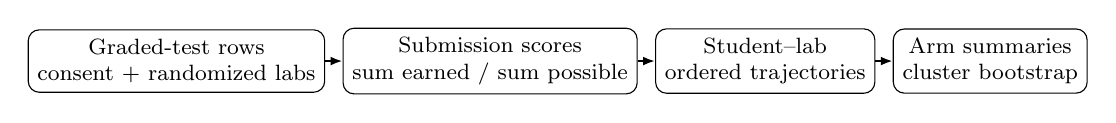
\begin{tikzpicture}[node distance=0.25cm and 0.22cm, every node/.style={draw,rounded corners,align=center,font=\footnotesize,minimum height=0.62cm}, arr/.style={-{Latex[length=1.5mm]},thick}]
\node (raw) {Graded-test rows\\consent + randomized labs};
\node (sub) [right=of raw] {Submission scores\\sum earned / sum possible};
\node (traj) [right=of sub] {Student--lab\\ordered trajectories};
\node (out) [right=of traj] {Arm summaries\\cluster bootstrap};
\draw[arr] (raw) -- (sub);
\draw[arr] (sub) -- (traj);
\draw[arr] (traj) -- (out);
\end{tikzpicture}
\caption{Analysis pipeline from ProgFeed test rows to student--lab outcomes.}
\label{fig:pipeline}
\end{figure}

\subsection{Estimation}
We report arm-specific means among initially failing units, retry rates, and eventual-full-credit rates. A percentile 95\% interval for mean $G_i$ is calculated from 5,000 bootstrap draws (seed 42), resampling students and retaining all of each selected student's observed labs. This preserves within-student clustering while matching the student--lab weighted point estimate. For arm a, the primary point estimate is the mean observed gain across initially failing units, as defined in Eq.~\ref{eq:armmean}. Table~\ref{tab:parameters} lists the fixed analysis settings. We do not report significance tests or causal contrasts: although assignment was randomized in the selected labs, this reanalysis conditions on an initial failure and uses final observed submissions; assignment also differs from actual feedback exposure.

\begin{equation}
\bar{G}_a=\frac{1}{n_a}\sum_{i:A_i=a,\,Y_{i1}<100} G_i.
\label{eq:armmean}
\end{equation}
\begin{table}[t]
\centering
\caption{Reproducible analysis settings}
\label{tab:parameters}
\small
\begin{tabular}{ll}
\toprule
Parameter & Setting \\
\midrule
Comparison labs & 05, 06, 07, 09 \\
Analysis unit & Student--lab \\
Primary outcome & Final minus first score after failure \\
Uncertainty & 5,000 student-cluster draws; seed 42 \\
Exposure & Assigned arm and delivered hint kept separate \\
\bottomrule
\end{tabular}
\end{table}

\section{Results and Discussion}\label{sec:results}
Table~\ref{tab:outcomes} summarizes 803 student--lab units across the three assigned arms; 280 units had a failed first attempt and form the outcome denominator for the displayed retry, full-credit, and gain measures. This table is descriptive. The natural-language arm has the largest observed mean gain (68.51 points), compared with 64.55 for no feedback and 63.19 for test-case hints. The corresponding student-cluster intervals overlap substantially. This pattern is compatible with the source paper's discussion that feedback format and validity may matter, but our restricted reaggregation is not a causal replication of its primary analyses~\cite{heickal2026}.

\begin{table*}[t]
\centering
\caption{Observed outcomes for student--lab units with a failed first submission}
\label{tab:outcomes}
\small
\begin{tabular}{lrrrrr}
\toprule
Assigned arm & Failed-first $n$ & Retry & Full credit & Mean gain (pp) & Cluster bootstrap 95\% CI\\
\midrule
No feedback & 93 & 97.8\% & 91.4\% & 64.55 & [58.48, 70.54]\\
Test-case hint & 91 & 95.6\% & 90.1\% & 63.19 & [56.16, 70.37]\\
Natural-language hint & 96 & 96.9\% & 92.7\% & 68.51 & [61.55, 74.83]\\
\bottomrule
\end{tabular}
\end{table*}

Fig.~\ref{fig:gain} visualizes the same score-gain estimates and student-cluster intervals. The point differences are modest relative to the intervals; overlapping intervals alone are not a formal test of equivalence or of a treatment effect. Nearly all initially failing units had a later submission, and about nine in ten reached full credit at least once. This high completion rate leaves limited room to distinguish arms using the binary full-credit measure. It also describes success at any observed attempt, not the quality of independent work after feedback is removed.

\begin{figure}[t]
\centering
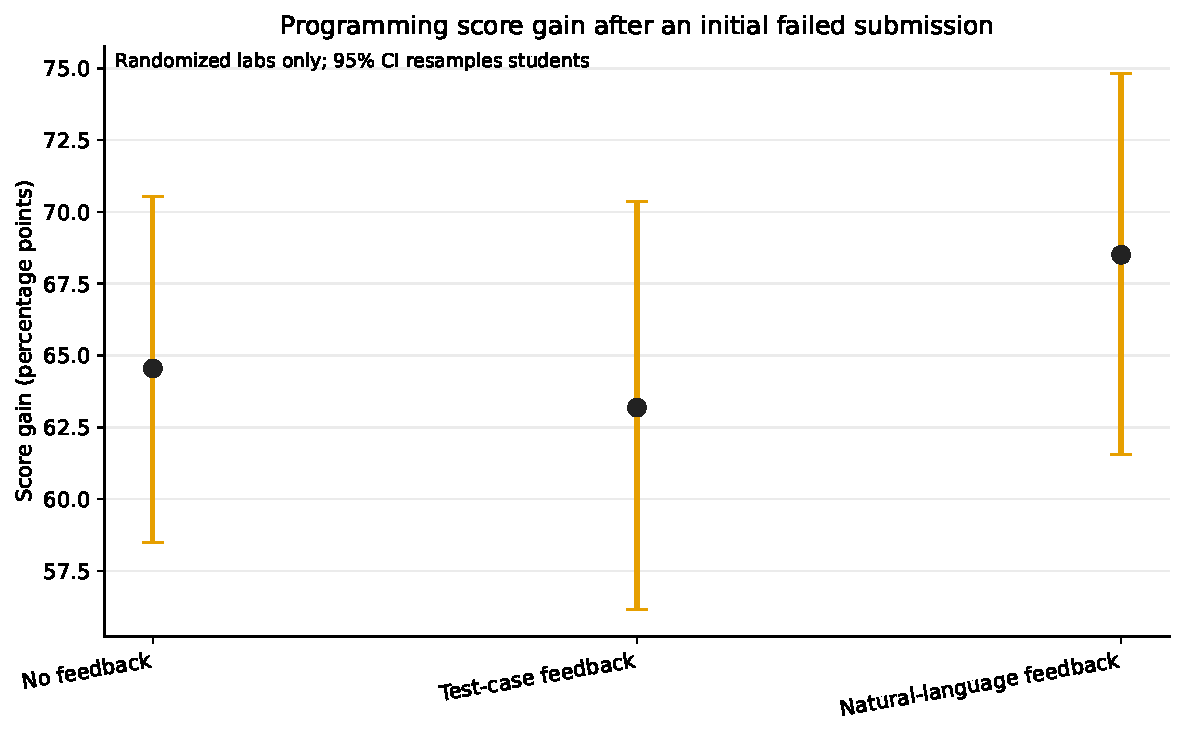
\includegraphics[width=\columnwidth]{../reports/figures/fig3_feedback_score_gain.pdf}
\caption{Mean score gain after an initial failure; intervals resample students.}
\label{fig:gain}
\end{figure}

The pattern is consistent with prior findings that feedback information content can change outcomes, while effects vary by intervention and context~\cite{hattie2007,wisniewski2020}. Natural-language feedback may help localize an error, whereas failing tests make the violated behavior explicit; neither format guarantees that a student can explain or reproduce a solution. Prior programming studies similarly caution that assisted performance and later learning are distinct outcomes~\cite{kazemitabaar2023,xue2024,sun2024}. Future experiments should measure independent post-tests, delayed retention, task transfer, and verified feedback validity, and should analyze assignment and actual hint exposure separately.

\section{Limitations and Conclusion}\label{sec:limits}
This study is a transparent reanalysis of one course and four randomized labs, not a new intervention. The public data contain no validated critical-thinking scale, delayed retention test, or transfer task. Conditioning on an initial failure may select different students or tasks across arms if assignment affects early attempts. Clustered intervals address dependence among repeated labs but not this selection or unmeasured lab difficulty. Point normalization cannot make assignments equally difficult, and the last observed submission is a censored endpoint. Hint correctness is also not measured uniformly for every assigned unit. The descriptive intervals do not remove these threats or warrant causal language.

Within this measurement envelope, all arms show high retry and eventual-full-credit rates, while the natural-language arm has a somewhat higher mean observed score gain. The estimates suggest hypotheses for a prospective study, not evidence that a feedback type improves durable learning. Future work should pre-register outcomes, preserve random assignment in analysis, record hint validity and exposure, and include unaided assessment. The source CSV is public and the repository supplies the pinned download and analysis scripts, supporting reproduction without committing student-level rows.

\bibliographystyle{IEEEtran}
\bibliography{task4_references}
\end{document}

